\chapter{Electrostatics, Part 1 (Point Charges)}
\label{chapter:electrostatics1}


\section{Review: The Charges Are}
We should already know a bit about charge particles:
\begin{itemize}
\item A \textbf{proton} carries a \textbf{positive} charge
\item An \textbf{electron} carries a \textbf{negative} charge
\item A \emph{net charge} of an object means an excess of protons or electrons
\item Similar charges are repel; opposite charges attract
\end{itemize}

\vspace{.2in}We start with electrostatics:
\begin{itemize}
\item Charges that are not moving relative to one another
\end{itemize}

The SI unit for electric charge is a \emph{coulomb}, which is the amount of
charges that flows through a circuit



\section{Coulomb's Law for Electrostatic Force}
\begin{center}
  \begin{tikzpicture}[scale=.65]
    \draw[vector,red] (0,0)--(2,0) node[right]{$\bm F_q$};
    \draw[vector,blue] (8,0)--(6,0) node[left] {$\bm F_q$};
    \shade[ball color=red] circle (.2) node[above]{$q_1$};
    \shade[ball color=blue] (8,0) circle (.2) node[above]{$q_2$};
    \draw[dashed] (0,0)--(0,-1.5);
    \draw[dashed] (8,0)--(8,-1.5);
    \draw[vector] (0,-1.3)--(8,-1.3) node[midway,below]{$\bm r_{12}$};
  \end{tikzpicture}
\end{center}
The \textbf{electrostatic force}\footnote{It is also known as the
\textbf{electric force} or \textbf{coulomb force} in different textbooks and
technical journals. We will use these terms interchangeably throughout the
course.} $\bm F_q$ is a mutually repulsive/attractive force between all
charged objects. The force that point charge $q_1$ exerts on $q_2$ is given
by \textbf{Coulomb's law}:

\begin{equation}
  \boxed{\bm F_q=\frac{kq_1q_2}{|\bm r_{12}|^2}\hat{\bm r_{12}}}
\end{equation}





\section{Coulomb's Law for Electrostatic Force}
\begin{equation}
  \boxed{
    \bm F_{12}=\frac{kq_1q_2}{|\bm r_{12}|^2}\hat{\bm r_{12}}
  }
\end{equation}
\begin{center}
  \begin{tabular}{l|c|c}
    \rowcolor{pink}
    \textbf{Quantity} & \textbf{Symbol} & \textbf{SI Unit} \\ \hline
    Electrostatic force    & $\bm F_{12}$ & \si\newton \\
    Coulomb's constant & $k$ &
    \si{\newton\metre\squared\per\coulomb\squared}\\
    Point charges 1 and 2  & $q_1$, $q_2$ &  \si\coulomb \\
    Distance between point charges & $|\bm r_{12}|$ & \si\metre \\
    Unit vector of direction between point charges & $\hat{\bm r_{12}}$ &
  \end{tabular}
\end{center}




\section{Coulomb's Constant}
\begin{equation}
  \boxed{\bm F_{12}=\frac{kq_1q_2}{|\bm r_{12}|^2}\hat{\bm r_{12}}}
\end{equation}

The constant $k$ in the Coulomb's law is called the
\textbf{coulomb's constant}, defined as:
\begin{equation}
  k=\dfrac1{4\pi\epsilon_0}=
  \SI{8.99e9}{\newton\metre\squared\per\coulomb\squared}
\end{equation}
where $\epsilon_0$ is a fundamental constant called the
\textbf{permittivity of free space}, or \textbf{vacuum permittivity}. It
measures a vacuum's ability to resist the formation of an electric field:
\begin{equation}
  \epsilon_0=\SI{8.85e-12}{C^2/N.m^2}
\end{equation}



\section{Coulomb's Law for Electrostatic Force}
\begin{center}
  \begin{tikzpicture}[scale=.5]
    \draw[vector,red] (0,0)--(2,0) node[right]{$\bm F_{12}$};
    \draw[vector,blue] (8,0)--(6,0) node[left] {$\bm F_{21}$};
    \shade[ball color=red] circle (.2) node[above]{$q_1$};
    \shade[ball color=blue] (8,0) circle (.2) node[above]{$q_2$};
    \draw[dashed] (0,0)--(0,-1.5);
    \draw[dashed] (8,0)--(8,-1.5);
    \draw[axes] (0,-1.3)--(8,-1.3) node[midway,below]{$\bm r_{12}$};
  \end{tikzpicture}
\end{center}
\begin{itemize}
\item Third law of motion: If $q_1$ exerts an electrostatic force
  $\bm F_{12}$ on $q_2$, then $q_2$ likewise exerts a force of
  $\bm F_{21}=-\bm F_{12}$ on $q_1$. The two forces are equal in magnitude
  and opposite in direction.
\item $q_1$ and $q_2$ are assumed to be \emph{point charges} that do not
  occupy any space
\item The scalar form is often used as well, since the direction of $F_q$ can
  easily be found:
  \begin{equation}
    \boxed{F_q=\frac{kq_1q_2}{r^2}}
  \end{equation}
\end{itemize}




\section{More Than One Charge}
\begin{center}
  \begin{tikzpicture}[scale=.4]
    \shade[ball color=red] circle (.72) node[white]{$Q$};
    
    \begin{scope}[rotate=45]
      \draw[vector,blue] (.72,0)--(2.5,0) node[right]{$\bm F_1$};
      \shade[ball color=blue] (7,0) circle (1) node[white]{$q_1$};
    \end{scope}
    
    \begin{scope}[rotate=105]
      \draw[vector,green] (.72,0)--(2,0) node[right]{$\bm F_2$};
      \shade[ball color=green] (4,0) circle (.65) node[white]{$q_2$};
    \end{scope}
    
    \begin{scope}[rotate=190]
      \draw[vector,yellow] (.7,0)--(3.5,0) node[above]{$\bm F_3$};
      \shade[ball color=yellow!70!black] (6,0) circle (1.1) node[white]{$q_3$};
    \end{scope}
    
    \begin{scope}[rotate=260]
      \draw[vector,violet] (.72,0)--(1.4,0) node[right]{$\bm F_4$};
      \shade[ball color=violet] (9,0) circle (.8) node[white]{$q_4$};
    \end{scope}
    
    \begin{scope}[rotate=125]
      \draw[->,ultra thick](.72,0)--(3.5,0) node[left]{$\bm F$};
    \end{scope}
  \end{tikzpicture}
 \end{center}
For a charge $Q$ that is subjected to the influence of multiple discrete
point charges $q_i$, the total electrostatic force that $Q$ experiences is
the vector sum of all the forces $\bm F_i$:

\begin{equation}
  \boxed{\bm F
    =\sum_i\bm F_i
    =kQ\left(\sum_{i=1}^N\frac{q_i}{r_i^2}\hat{\bm r_i}\right)
  }
\end{equation}
  




\section{Continuous Distribution of Charges}
As $N\rightarrow\infty$, the summation becomes an integral, and can now be
used to describe the force from charges with \emph{spatial extend} i.e.\
charges that take up physical space (e.g.\ a continuous distribution of
charges):
\begin{equation}
  \boxed{\bm F
    =\int\dl\bm F
    =kQ\int\frac{\dl q}{r^2}\hat{\bm r}
  }
\end{equation}




\section{Infinitesimal Charge $\dl q$}
\label{section:charge-density}

Expressions for infinitesimal charge $\dl q$ is similar to the infinitesimal
mass $\dl m$ concept discussed earlier in the course (Class 5:
Center of Mass, and Class 7: Rotational Motion)
\begin{itemize}
\item Linear charge density (for 1D problems)
  \begin{equation}
    \gamma = \diff qL\quad\rightarrow\quad \dl q =\gamma\dl L
  \end{equation}
  \item Surface charge density (for 2D problems)
    \begin{equation}
      \sigma=\diff qA\quad\rightarrow\quad \dl q=\sigma\dl A
    \end{equation}
  \item Charge density (for 3D problems)
    \begin{equation}
      \rho=\diff qV\quad\rightarrow\quad \dl q=\rho\dl V
    \end{equation}
\end{itemize}


    
\section{Electric Field}
The expression for \textbf{electric field} is obtained by repeating the same
procedure as with gravitational field, by grouping the variables in
Coulomb's law:
\begin{equation}
  F_q
  =\underbrace{
    \left[\frac{kq_1}{|\bm r_{12}|^2}\hat{\bm r}\right]
  }_{\bm E}q_2
\end{equation}
The electric field $\bm E$ created by $q_1$ is a vector function (called a
\textbf{vector field}) that shows how it influences other charged particles
around it.




\section{Electric Field Near a Point Charge}
The electric field a distance $r$ away from a point charge $q$ is given by:
\begin{equation}
  \boxed{\bm E(q,\bm r)=\frac{kq}{r^2}\hat{\bm r}}
  \label{eq:pt-charge-E}
\end{equation}
\begin{center}
  \begin{tabular}{l|c|c}
    \rowcolor{pink}
    \textbf{Quantity} & \textbf{Symbol} & \textbf{SI Unit} \\ \hline
    Electric field intensity    & $\bm E$ & \si{\newton\per\coulomb}\\
    Coulomb's constant          & $k$   & \si{N.m^2/C^2} \\
    Source charge               & $q$   & \si\coulomb \\
    Distance from source charge & $r$ & \si\metre \\
    Radially outward direction from point source & $\hat{\bm r}$ &
  \end{tabular}
\end{center}
The direction of $\bm E$ is radially outward from a positive point charge
and radially inward toward a negative charge. The SI unit for electric field
is \textbf{newton per coulomb} (\si{\newton\per\coulomb}) or
\textbf{volt per meter} (\si{\volt\per\metre}). Both units are equivalent,
and both are used in AP exams.




\section{More Than One Charge}
When multiple discrete point charges are present, the total electric field at
any position $\bm r$ is the vector sum of all the fields $\bm E_i$:
\begin{equation}
  \boxed{\bm E
    =\sum_i\bm E_i
    =k\left(\sum_{i=1}^N\frac{q_i}{r_i^2}\hat{\bm r_i}\right)
  }
\end{equation}
As $N\rightarrow\infty$, the summation becomes an integral, and can now be
used to describe the electric field generated by \emph{charge distributions
with spatial extend}:
\begin{equation}
  \boxed{
    \bm E=\int\dl\bm E=k\int\frac{\dl q}{r^2}\hat{\bm r}
  }
\end{equation}
In general, this integral is difficult to evaluate for complex geometries,
but in AP Physics C, we can usually exploit symmetry.




\section{Think Electric Field}
$\bm E$ itself \emph{doesn't do anything} until another charge interacts with
it. And when there is a charge $q$, the electrostatic force $\bm F_q$ that
the charge experiences is proportional to $q$ and $\bm E$, regardless of how
the electric field is generated\footnote{Analogous to the relationship
for gravity: $\bm F_g=m\bm g$}:
\begin{equation}
  \boxed{\bm F_q=q\bm E}
\end{equation}
A positive charge in the electric field experiences an electrostatic force
$\bm F_q$ in the same direction as $\bm E$; a negative charge experiences
a force in the opposite direction as $\bm E$.




\section{Electric Field Lines}
\textbf{Electric field lines} can be used to visualize the direction of the
electric field. For point charges:
\begin{center}
  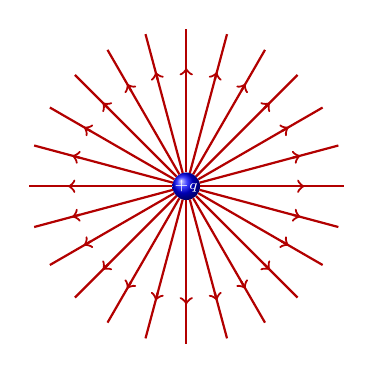
\begin{tikzpicture}[scale=.5]
    \shade[ball color=blue] circle (.35) node[white]{\tiny $+q$};
    \foreach \theta in {15,30,...,360}{
      \begin{scope}[rotate=\theta,red!70!black,thick]
        \draw[->] (.35,0)--(3,0);
        \draw (2.8,0)--(4,0);
      \end{scope}
    }
  \end{tikzpicture}
  \hspace{.2in}
  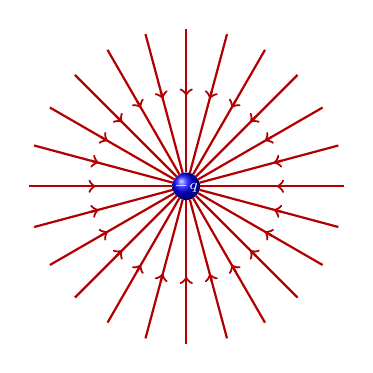
\begin{tikzpicture}[scale=.5]
    \shade[ball color=blue] circle (.35) node[white]{\tiny $-q$};
    \foreach \theta in {15,30,...,360}{
      \begin{scope}[rotate=\theta,red!70!black,thick]
        \draw (.35,0)--(2.5,0);
        \draw[<-] (2.3,0)--(4,0);
      \end{scope}
    }
  \end{tikzpicture}
\end{center}




\section{Electric Field from Multiple Charges}
\begin{center}
  \pic{.8}{../electrostatics/field-lines}
\end{center}
\begin{itemize}
\item Electric field lines must begin and/or end at a charge
\item Field lines do not cross
\item Direction of the electric field is tangent to the field lines
\end{itemize}




\section{Lord of the Ring Charge}
Suppose you have been given \emph{The One Ring To Rule Them All}, and you
found out that it is charged! What is its electric field at point $P$ along
its axis?
\begin{center}
  \pic{.5}{../electrostatics/physicsbook_emism_graphik_35}
\end{center}
Note that calculating the electric field away from the axis is very
difficult.




\section{Electric Field Along Axis of a Ring Charge}

\begin{center}
  \pic{.5}{../electrostatics/Fig25}
\end{center}

\begin{itemize}
\item We can separate the electric field $\dl\bm E$ (generated by charge
  $\dl q$) into axial ($\dl E_x$) and radial ($\dl E_\perp$) components
\item Based on symmetry, $\dl E_\perp$ doesn't contribute to anything; but
  $\dl E_x$ is pretty easy to find:
\end{itemize}
\begin{equation}
  \dl E_x =\frac{k\dl q}{r^2}{\color{red}\cos\theta}
  =\frac{k\dl q}{r^2}{\color{red}\frac xr}
  =\frac{kx\dl q}{(x^2+a^2)^{3/2}}
\end{equation}
Integrating this over all charges $\dl q$, we have:
\begin{equation} 
    E_x          
    =\int \dl E_x       
    =\frac{kx}{(x^2+a^2)^{3/2}}\int \dl q=\boxed{\frac{kQx}{(x^2+a^2)^{3/2}}}
\end{equation}                     




\section{Electric Field Along Axis of a Uniformly Charged Disk}
Let's extend what we know to a disk of radius $a$ and charge density $\sigma$
\begin{center}
  \pic{.5}{../electrostatics/serway}
\end{center}
  
We start with the solution from the ring problem, and replace $Q$ with
$\dl q=2\pi\sigma r\dl r$:
\begin{equation}
  \dl E_x =\frac{2\pi kr\sigma x}{(x^2+r^2)^{3/2}}\dl r
\end{equation}
Integrating over the entire disk:
\begin{equation}
  E_x =\pi kx\sigma\int_0^a\frac{2r}{(x^2+r^2)^{3/2}}\dl r
\end{equation}
This is not an easy integral!

Luckily for us, the integral is in the form of $\int u^n\dl u$,
with $u=x^2+r^2$ and $n=\frac{-3}2$. You can find the integral in any math
textbook:

\begin{equation}
  E_x =2\pi k\sigma\left(1-\frac x{\sqrt{x^2+a^2}}\right)
\end{equation}
  

\section{Electric Potential Energy}
The electrostatic force is a conservative force; the work done by $\bm F_q$
is related to the change in \textbf{electric potential energy} $U_q$:

\begin{equation}
  W_q=\int\bm F_q\cdot\dl\bm r
  =kq_1q_2\int_{r_0}^{r_1}\frac{\dl r}{r^2}
  =-\frac{kq_1q_2} r\Big|^{r_1}_{r_0}=-\Delta U_q
\end{equation}
$U_q$ is the energy stored between a system of two charges, defined as:
\begin{equation}
  \boxed{U_q=\frac{kq_1q_2} r}
\end{equation}
\fcolorbox{black}{yellow!5}{
  \begin{minipage}{.97\linewidth}
    \begin{itemize}
    \item Positive work done by electrostatic force decreases $U_q$, while
    \item Negative work done by electrostatic force increases $U_q$
    \item $W_q$ depends on $r_0$ and $r_1$, but not \emph{how} the charge
      moves from $r_0\rightarrow r_1$
    \item Only work done by $\bm F_q$ can change $U_q$
    \end{itemize}
  \end{minipage}
}




\section{How it Differs from Gravitational Potential Energy}
$U_q$ can be ($+$) or ($-$), because charges can be either ($+$) or ($-$)

Two positive charges:

\begin{equation}
  U_q>0
\end{equation}
    
Two negative charges:

\begin{equation}
  U_q>0
\end{equation}
    
One positive and one negative charge:

\begin{equation}
  U_q<0
\end{equation}
  
\begin{itemize}
\item $U_q>0$ (both charges have the same sign): work is done to bring two
  charges together from $r=\infty$ to $r$
\item $U_q<0$ (the charges are opposite signs): work is done to separate the
  two charges from $r$ to $r=\infty$
\item Gravitational potential $U_g$ is always $<0$ because mass can only be
  positive
\end{itemize}




\section{Relating $U_q$ to $\bm F_q$}
From the fundamental theorem calculus, we can relate electrostatic force
($\bm F_q$) to electric potential energy ($U_q$) by the gradient operator:

\begin{equation}
  U_q=-\int\bm F_q\cdot\dl\bm r\quad\rightarrow\quad
  \bm F_q(r)=-\nabla U_q=-\diffp{U_q}r\hat{\bm r}
\end{equation}
Electrostatic force $\bm F_q$ always points from high to low potential
energy (steepest descent direction)




\section{Potential Energy with More Than Two Charges}
When there are more than two charges, the total potential energy is the
total between the systems of 2 charges:

\begin{center}
  \begin{tikzpicture}[scale=1.3]
    \draw (0,0)--(1,-2) node[midway,right]{$r_3$}
    --(-3,-2) node[midway,below]{$r_2$} -- (0,0) node[midway,left=3]{$r_1$};
    \draw[mass] circle (.2) node{$q_1$};
    \draw[mass] (1,-2) circle (.2) node{$q_3$};
    \draw[mass] (-3,-2) circle (.2) node{$q_2$};
  \end{tikzpicture}
\end{center}

\begin{equation}
  U_q=\frac{kq_1q_2}{r_1} +\frac{kq_2q_3}{r_2} +\frac{kq_1q_3}{r_3}
\end{equation}
The energy stored can be either positive or negative depending on the sign of
the charges of $q_1$, $q_2$ and $q_3$.


\fcolorbox{black}{yellow!10}{
  \begin{minipage}{.97\linewidth}
    \textbf{Example:} Four identical charges $q$ are located at the four corners
    of a square of length $L$. What is the total potential energy of the system?
    \begin{center}
      \begin{tikzpicture}[scale=1.3]
        \draw rectangle (2,2) node[midway,above=35]{$L$};
        \draw[mass] (0,2) circle (.15) node{$q$};
        \draw[mass] (0,0) circle (.15) node{$q$};
        \draw[mass] (2,0) circle (.15) node{$q$};
        \draw[mass] (2,2) circle (.15) node{$q$};
      \end{tikzpicture}
    \end{center}
  \end{minipage}
}




\section{Electric Potential}

An object at a specific location inside a gravitational field has a
gravitational potential energy proportional to its mass, i.e.\
\begin{equation}
    U_g=V_gm
\end{equation}
This ``constant'' $V_g$ is called the \textbf{gravitational potential}, which
is defined as \emph{gravitational potential energy per unit mass}. In the
simple case with a uniform gravitational field:
\begin{equation}
  V_g(h)=\frac{U_g}m=gh
\end{equation}
In the general case for the gravitational potential energy stored between
$M$ and $m$, we can define the gravitational potential from ``source mass''
$M$:
\begin{equation}
  V_g=\frac{U_g}m=-\frac{GM}r
\end{equation}
When $m$ is in this potential $V_g$, the gravitational potential energy is:
\begin{equation}
  U_g=V_gm=-\frac{GMm}r
\end{equation}
In agreement with the previous equations


This is also true for a charged particle $q$ in an electric field
created by $q_s$. In this case, the potential (the ``constant'') is called the
\textbf{electric potential}. The unit for electric potential is a \emph{volt}
which is \emph{one joule per coulomb}, i.e.\
$\SI1\volt=\SI1{\joule\per\coulomb}$
\begin{equation}
  \boxed{
    V=\frac{U_q}q
  }
\end{equation}
The electric potential from a source \underline{\emph{point}} charge $q_s$ is
therefore:
\begin{equation}
  \boxed{
    V=\frac{kq_s}r
  }
\end{equation}




\section{Electric Potential: Point Charges}
  
\begin{center}
  \centering
  \begin{tikzpicture}[scale=.75]
    \shade[ball color=blue] circle (.3) node[white]{\tiny$\bm{+q}$};
    \foreach \theta in {20,40,...,360}{
      \draw[rotate=\theta,axes,gray] (.3,0)--(3,0);
      \draw[rotate=\theta,thick,gray] (2.8,0)--(4,0);
    }
    \foreach \r in {1,2,3}{
      \draw[very thick,red] circle (\r);
      \node[red,below] at (0,-\r+.09){$V_\r$};
    }
  \end{tikzpicture}
\end{center}

For a point charge $q$, every point at a distance $r$ has the same
electric potential $V$.
\begin{itemize}
\item The red lines have the same electric potential; they are called
  \textbf{equipotential lines}, or \textbf{equipotential contours}
\item Equipotential lines are perpendicular to the electric field lines
\item Electric field lines always points from higher $V$ toward lower $V$
\end{itemize}
\begin{equation}
  V_1>V_2>V_3
\end{equation}
  
  %\vspace{.1in}In AP Physics C, equipotential contours are sometimes also known
  %as \textbf{isolines of equal electric potential}.




\section{Electric Potential}
  
\begin{center}
  \centering
  \begin{tikzpicture}[scale=.75]
    \shade[ball color=blue] circle (.3) node[white]{\tiny$\bm{+q}$};
    \foreach \theta in {20,40,...,360}{
      \draw[rotate=\theta,axes,gray] (.3,0)--(3,0);
      \draw[rotate=\theta,gray,thick] (2.8,0)--(4,0);
    }
    \foreach \r in {1,2,3}{
      \draw[very thick,red] circle (\r);
      \node[red,below] at (0,-\r+0.09){$V_\r$};
    }
    \shade[ball color=red,rotate=-20] (2,0) circle (.23) node[white]{$Q$};
  \end{tikzpicture}
\end{center}
A charge $Q$ that is placed inside this electric field has an electric
potential energy of:
\begin{equation}
  U_q=QV=Q\left[\frac{kq}r\right]
\end{equation}  
in agreement with equation for electric potential energy
  





\section{Electric Potential from Multiple Charges}
When multiple discrete point charges are present, the total electric
potential is given by the summation\footnote{Note that this is scalar
summation!}:

\begin{equation}
  \boxed{
    V =k\sum_{i=1}^N\frac{q_i}{r_i}
  }
\end{equation}
As $N\rightarrow\infty$, the summation becomes an integral, and we can use it
to evaluate the potential from a continuous distribution of charges:
\begin{equation}
  \boxed{
    V =k\int\frac{\dl q}r
  }
\end{equation}
  %where $r$ is the distance to the infinitesimal charge $\dl q$




\fcolorbox{black}{yellow!10}{
  \small
  \begin{minipage}{.97\linewidth}
    \begin{center}
      \begin{tikzpicture}
        \draw[axes] (-2,0)--(2,0) node[right]{$x$};
        \draw[axes] (0,-2)--(0,2) node[right]{$y$};
        \draw[gray] circle (1.5);
        \draw[line width=2,red,rotate=90] (1.5,0) arc (0:180:1.5)
        node[pos=.25,above=3]{$Q$};
      \end{tikzpicture}
    \end{center}
    \textbf{Example:} A uniform charge $Q$ is located
    \begin{enumerate}[nosep]
      %\item What is the electric field at the origin?
    \item What is the electric potential at the origin?
    \item A charge $q$ is moved from $x=\infty$ to the origin. What is the
      work done?
    \end{enumerate}
  \end{minipage}
}
  




\section{Relating $V$ to $\bm E$}
In the same way that the fundamental theorem of calculus relates the 
electrostatic force ($\bm F_q$) and electric potential energy ($U_q$) by the
gradient operator, electric field ($\bm E$) and electric potential ($V$) are
also related the same way:

\begin{equation}
  V(r)=-\int\bm E(r)\cdot\dl\bm r\quad\rightarrow\quad
  \bm E(r)=-\nabla V(r)=-\diff Vr\hat{\bm r}
\end{equation}
\begin{itemize}
\item Electric field $\bm E$ always points from high to low electric
  potential
\item Electric field is also called ``potential gradient''
\end{itemize}





\section{Electric Potential Difference}
\begin{center}
  
  \begin{tikzpicture}[scale=.75]
    \shade[ball color=blue] circle (.3) node[white]{$Q$};
    \foreach \theta in {30,60,...,360}{
      \draw[rotate=\theta,axes,gray] (.3,0)--({7-4*sin(\theta/2)},0);
    }
    \draw[red,ultra thick,dotted,<-]
    (2.5*cos{30}+.23,-2.5*sin{30}) to[out=0,in=270](5*cos{15},5*sin{15}-.2);
    \draw[thick,red,rotate=-70] (2.5,0) arc (0:100:2.5) node[above]{$V_2$};
    \draw[thick,red,rotate=-60] (5,0) arc (0:90:5) node[above]{$V_1$};
    \begin{scope}[rotate=-30]
      \shade[ball color=red](2.5,0) circle (.23) node[white]{$q$};
      \draw[<->,thick] (.3,0)--(2.27,0) node[midway,above]{$r_2$};
    \end{scope}
    \begin{scope}[rotate=15]
      \shade[ball color=red] (5,0) circle (.23) node[white]{$q$};
      \draw[<->,thick] (.3,0)--(4.77,0) node[pos=2/3,below]{$r_1$};
    \end{scope}
  \end{tikzpicture}
\end{center}
When a charge moves from $r_1$ to $r_2$, the change in electric potential
energy is related to the change in electric potential by:
\begin{equation}
  \Delta U_q=U_2-U_1=q\Delta V
\end{equation}
where $\Delta V$ is called the \textbf{potential difference}
  





\section{Potential Difference (Voltage)}
The change in electric potential is called the
\textbf{electric potential difference} or \textbf{voltage}:
\begin{equation}
  \boxed{\Delta V=\frac{\Delta U_q}q}\quad\textsf{\normalsize and}\quad
  \boxed{\dl V=\frac{\dl U_q}q}
\end{equation}
Here, we can relate $\Delta V$ to an equation that we knew from Physics 11
and AP Physics 2, which related to the energy dissipated in a resistor in a
circuit $\Delta U$ to the voltage drop $\Delta V$:
\begin{equation}
  \boxed{\Delta U_q=q\Delta V}
\end{equation}
Electric potential difference also has the unit \emph{volts} (\si\volt)




\section{Relating $V$ and $\Delta V$}
Electric potential $V(r)$, a furnction of space, is related to the electric
field $E$ by an {\color{red}indefinite} integral:
\begin{equation}
  V{\color{red}(r)}=-\int\bm E(\bm r)\cdot\dl\bm r
\end{equation}
Whereas electric potential difference is related to the electric field $E$
by a {\color{blue}definite} integral from $r_0$ to $r_1$, with a definite
value:
\begin{equation}
  {\color{blue}\Delta} V
  =-\int_{\bm r_0}^{\bm r_1}
  \bm E(\bm r)\cdot\dl\bm r
\end{equation}




\section{Getting Those Names Right}
Remember that these three scalar quantities, as opposed to electrostatic
force $\bm F_q$ and electric field $\bm E$ which are vectors
\begin{itemize}
\item Electric potential energy:
  \begin{equation}
    U_q=\frac{kq_1q_2}r
  \end{equation}
  \item Electric potential:

    \begin{equation}
      V=\frac{U_q}q
    \end{equation}
  \item Electric potential difference (voltage):
    \begin{equation}
      \Delta V=\frac{\Delta U_q}q
    \end{equation}
  \end{itemize}




%\section{Equipotential Lines}
%  \begin{center}
%    \pic{.65}{plate3}
%  \end{center}
%  The dotted blue lines are called \textbf{equipotential lines}. They are
%  always \emph{perpendicular} to the electric field lines. Charges moving in
%  the direction of the equipotential lines have constant electric potential

